\documentclass[tikz,border=2pt]{standalone}
\usepackage{amsmath,amssymb}
\usepackage{pgfplots}
\pgfplotsset{compat=1.18}

\begin{document}
% Bin(100, 0.2) with the N(20, 16) density, which has the same mean np = 20 and variance
% np(1-p) = 16. The upper tail P(X >= 25) corresponds to the normal area beyond 24.5.
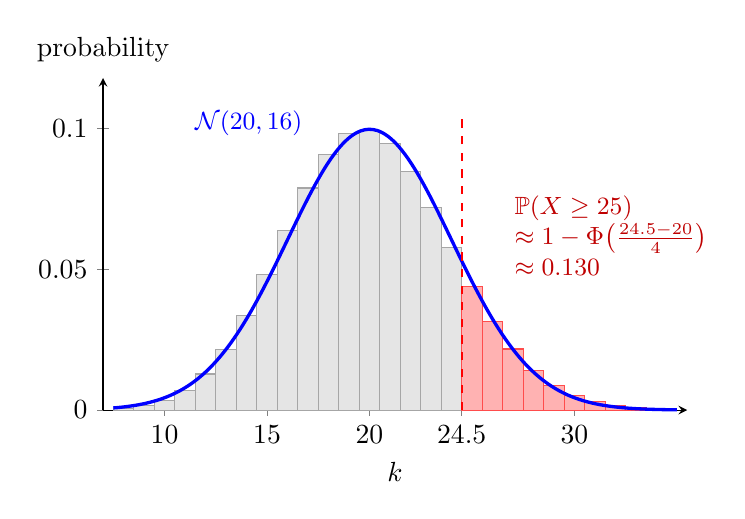
\begin{tikzpicture}
	\begin{axis}[
		axis lines=left, xmin=7, xmax=35.5, ymin=0, ymax=0.118,
		xtick={10,15,20,24.5,30}, xticklabels={$10$,$15$,$20$,$24.5$,$30$}, ytick={0,0.05,0.1},
		yticklabel style={/pgf/number format/fixed, /pgf/number format/precision=2}, scaled y ticks=false,
		xlabel={$k$}, ylabel={probability}, ylabel style={rotate=-90, anchor=south, at={(axis description cs:0,1.02)}},
		width=9cm, height=5.8cm, clip=false
		]
		\addplot[ybar, bar width=1, fill=gray!20, draw=gray!70] coordinates {(8,0.0006) (9,0.0015) (10,0.0034) (11,0.0069) (12,0.0128) (13,0.0216) (14,0.0335) (15,0.0481) (16,0.0638) (17,0.0789) (18,0.0909) (19,0.0981) (20,0.0993) (21,0.0946) (22,0.0849) (23,0.0720) (24,0.0577)};
		\addplot[ybar, bar width=1, fill=red!30, draw=red!70] coordinates {(25,0.0439) (26,0.0316) (27,0.0217) (28,0.0141) (29,0.0088) (30,0.0052) (31,0.0029) (32,0.0016) (33,0.0008) (34,0.0004)};
		\addplot[blue, very thick, domain=7.5:35, samples=140, smooth] {exp(-(x-20)^2/32)/(4*sqrt(2*pi))};
		\draw[red, dashed, thick] (axis cs:24.5,0) -- (axis cs:24.5,0.105);
		\node[blue, anchor=south east, font=\small] at (axis cs:17.2,0.094) {$\mathcal{N}(20,16)$};
		\node[red!75!black, anchor=west, font=\small, align=left] at (axis cs:26.6,0.062) {$\mathbb{P}(X\ge25)$\\ $\approx1-\Phi\big(\tfrac{24.5-20}{4}\big)$\\ $\approx0.130$};
	\end{axis}
	
\end{tikzpicture}
\end{document}
